% Provenance (never printed): old seconde/premiere S material on the
% atmosphere (storms, cyclones, the energy of the water cycle) and the
% natural-hazard themes of SVT; see sources/book2/PROVENANCE.md. Tracks,
% genesis statistics and the pressure--wind relation are computed in
% figdata/grade-10/cyclones.py from IBTrACS v04r01; the surge, thunder and
% energy numbers in the same script.
\chapter{Tormentas y ciclones tropicales}\label{ch:g10:storms-and-cyclones}

Una calurosa tarde de verano termina en tormenta. El cielo se oscurece, una
ráfaga de viento frío barre la calle, un relámpago ilumina las nubes, y
empiezas a contar: uno, dos, tres, \ldots{} nueve segundos después retumba el
trueno. La tormenta está a unos tres kilómetros. Dentro de una hora habrá
pasado, y el aire estará fresco y limpio. Sobre los cálidos océanos
tropicales, los mismos ingredientes ---aire cálido y húmedo que sube y se
condensa--- pueden organizarse en tempestades de un tamaño completamente
distinto: los ciclones tropicales, de cientos de kilómetros de diámetro, que
duran días y traen vientos capaces de arrasar bosques y una subida del mar
que inunda costas enteras. Este capítulo estudia las tormentas, los \omterm{def:g10:storms-and-cyclones:tornado}{tornados}
y los ciclones tropicales, y de dónde sacan su energía.

\begin{safety}
Si oyes truenos, un \omterm{def:g10:storms-and-cyclones:lightning}{rayo} puede alcanzarte. Entra en un edificio o en un coche
cerrado y quédate dentro hasta bastante después del último trueno. No te
refugies nunca bajo un árbol aislado, y aléjate de las cimas, de los campos
abiertos y del agua.
\end{safety}

\begin{recall}
Las masas de aire, los frentes, las borrascas (zonas de baja presión) y los
anticiclones se dibujan en los mapas del tiempo con isobaras, líneas de
igual presión (Libro 1, año 8). Un peligro natural es un fenómeno natural
que puede dañar a las personas y lo que construyen (Libro 1, año 5). El
sonido se propaga en el aire a unos \qty{340}{m/s}, y la luz de forma casi
instantánea (los libros de física). El aire cálido y húmedo que sube se
enfría, se condensa en nube al llegar a su \omterm{def:g10:why-clouds-form:condensation-level}{nivel de condensación} y libera
\omterm{def:g10:earth-energy-budget:latent-heat}{calor latente}; el aire saturado suele ser inestable
(\cref{ch:g10:why-clouds-form}).
\end{recall}

\section{Las tormentas}

\begin{definition}[Tormenta eléctrica]\label{def:g10:storms-and-cyclones:thunderstorm}
Una \emph{tormenta eléctrica}\index{tormenta electrica@tormenta eléctrica}
es una tormenta producida por una nube de tipo cumulonimbo, con \omterm{def:g10:storms-and-cyclones:lightning}{rayos} y
truenos, normalmente con chubascos intensos y rachas de viento, y a veces
con granizo.
\end{definition}

Una tormenta nace de un \omterm{def:g10:why-clouds-form:stability}{aire inestable} y húmedo. En su primera fase, un
cúmulo crece hacia arriba, alimentado por una fuerte corriente ascendente;
la condensación libera \omterm{def:g10:earth-energy-budget:latent-heat}{calor latente} y mantiene el aire que sube más
caliente que su entorno. En su fase de madurez, la nube llega al \omterm{def:g10:why-clouds-form:stability}{aire
estable} de las capas altas y se extiende en un yunque; las gotas y los
granizos crecen lo suficiente para caer, y la lluvia que cae arrastra aire
frío consigo: una corriente descendente que se extiende junto al suelo como
un frente de racha frío. En su última fase, la corriente descendente ocupa
toda la nube, corta el aporte de aire cálido y húmedo, y la tormenta se
agota lloviendo.

\begin{omfigure}
\begin{tikzpicture}[font=\footnotesize, >={Stealth[length=2mm]}]
  \foreach \dx/\title in {0/{1. desarrollo}, 4.6/{2. madurez}, 9.2/{3. disipación}}
    \node[anchor=north] at (\dx+1.6,-0.15) {\title};
  \draw[thick, black!60] (-0.3,0) -- (12.9,0);
  % stage 1: a tall cumulus
  \pic[scale=1.4, transform shape] at (1.6,1.2) {puffycloud};
  \pic[scale=1.1, transform shape] at (1.6,2.0) {puffycloud};
  \foreach \x in {1.2,1.6,2.0} \draw[->, thick, omThm!80!black] (\x,0.2) -- (\x,2.6);
  % stage 2: cumulonimbus with anvil
  \fill[black!8, draw=black!50] (5.0,1.0) -- (4.9,4.0) -- (4.2,4.4) -- (8.0,4.6) -- (7.4,4.0) -- (7.2,1.0) -- cycle;
  \draw[->, thick, omThm!80!black] (5.5,0.2) -- (5.5,4.2);
  \draw[->, thick, omThm!80!black] (5.9,0.2) -- (5.9,4.2);
  \draw[->, thick, omDef!80!black] (6.7,3.4) -- (6.7,0.3) -- (7.6,0.3);
  \foreach \x in {6.4,6.85,7.05} \draw[omDef!50] (\x,0.95) -- (\x-0.1,0.1);
  \node[anchor=west, align=left] at (8.0,4.6) {yunque};
  \node[anchor=west, align=left, omDef!80!black] at (7.65,0.45) {frente de racha};
  % stage 3: dissipating
  \fill[black!8, draw=black!50] (9.7,1.2) -- (9.6,3.6) -- (9.0,4.0) -- (12.6,4.1) -- (12.0,3.6) -- (11.8,1.2) -- cycle;
  \foreach \x in {10.3,10.9,11.5} \draw[->, thick, omDef!80!black] (\x,3.2) -- (\x,0.3);
  \foreach \x in {10.6,11.2} \draw[omDef!50] (\x,1.15) -- (\x-0.1,0.1);
  % legend
  \draw[->, thick, omThm!80!black] (0,5.0) -- (0,5.5); \node[anchor=west] at (0.1,5.25) {corriente ascendente cálida};
  \draw[->, thick, omDef!80!black] (3.2,5.5) -- (3.2,5.0); \node[anchor=west] at (3.3,5.25) {corriente descendente fría};
\end{tikzpicture}

{\small Las tres fases de una tormenta (esquema, sin escala): un cúmulo en
desarrollo alimentado por corrientes ascendentes; el cumulonimbo maduro, con
su yunque, su corriente ascendente y una corriente descendente arrastrada
por la lluvia; la tormenta en disipación, toda ella corriente descendente.}
\end{omfigure}

Dentro de la nube, los choques entre partículas de hielo que el aire sube y
baja separan cargas eléctricas: la nube se carga, normalmente de forma
negativa en su parte baja y positiva en su parte alta, y el suelo que hay
debajo adquiere una carga propia.

\begin{definition}[Rayo]\label{def:g10:storms-and-cyclones:lightning}
Un \emph{rayo}\index{rayo} es una chispa eléctrica gigante que descarga
regiones cargadas de una tormenta, dentro de la nube, entre nubes o entre la
nube y el suelo. Calienta un estrecho canal de aire de forma tan brusca que
el aire se dilata con una onda de choque: el sonido de esta dilatación es el
\emph{trueno}.
\end{definition}

\begin{omfigure}
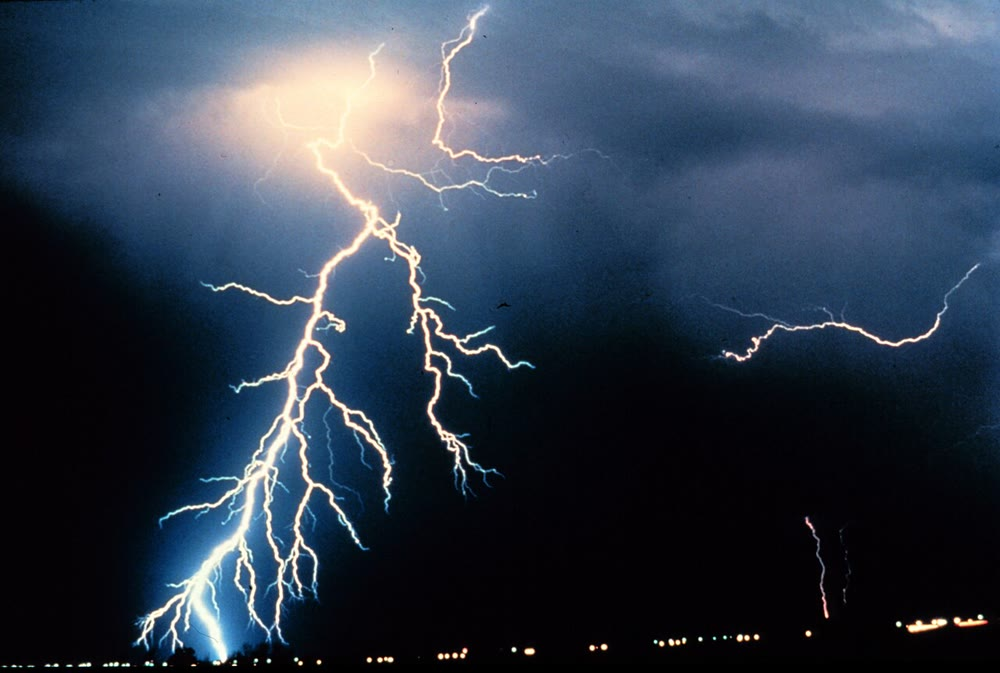
\includegraphics[width=0.62\linewidth]{images/book2/g10-noaa-lightning.jpg}

{\small \omterm{def:g10:storms-and-cyclones:lightning}{Rayos} entre nubes y de la nube al suelo durante una tormenta
nocturna. Fotografía: C.~Clark, NOAA National Severe Storms Laboratory
(dominio público).}
\end{omfigure}

Los satélites que cuentan los destellos de luz sobre todo el planeta
registran unos 1400 millones de \omterm{def:g10:storms-and-cyclones:lightning}{rayos} al año, es decir, 44 cada segundo.
% ledger: christian:flash-rate

\begin{method}[Distancia de una tormenta entre el relámpago y el trueno]\label{met:g10:storms-and-cyclones:distance}
\begin{enumerate}
  \item La luz del relámpago llega prácticamente en el acto; el trueno
        viaja a la velocidad del sonido, unos \qty{343}{m/s} a
        \qty{20}{\degreeCelsius}.
  \item Cuenta los segundos $t$ que pasan entre el relámpago y el trueno.
  \item La distancia es de $343\,t$ metros: alrededor de \qty{1}{km} por
        cada tres segundos.
\end{enumerate}
\end{method}
% ledger: const:R, earth:Mmol (speed of sound computed in figdata/grade-10/cyclones.py)

\section{Los tornados}

\begin{definition}[Tornado]\label{def:g10:storms-and-cyclones:tornado}
Un \emph{tornado}\index{tornado} es una columna de aire en rotación violenta,
en contacto con el suelo, que cuelga de la base de un cumulonimbo.
\end{definition}

Los \omterm{def:g10:storms-and-cyclones:tornado}{tornados} más fuertes nacen de \emph{supercélulas}, tormentas cuya
corriente ascendente gira en bloque. Un \omterm{def:g10:storms-and-cyclones:tornado}{tornado} es pequeño y breve: suele
medir unos cientos de metros de diámetro, dura minutos y recorre por
término medio unos \qty{5.6}{km}. Pero sus vientos son los más fuertes de la
superficie terrestre: un radar móvil midió unos \qty{135}{m/s} (unos
\qty{480}{km/h}) por encima del suelo en un \omterm{def:g10:storms-and-cyclones:tornado}{tornado} de Oklahoma en mayo de
1999. Estados Unidos tiene más \omterm{def:g10:storms-and-cyclones:tornado}{tornados} que ningún otro país, unos 1200 al
año; otras regiones donde son frecuentes son las praderas canadienses,
Bangladés, el norte de Argentina y el sur de Brasil, y Gran Bretaña.
% ledger: spc:tornado

\begin{omfigure}
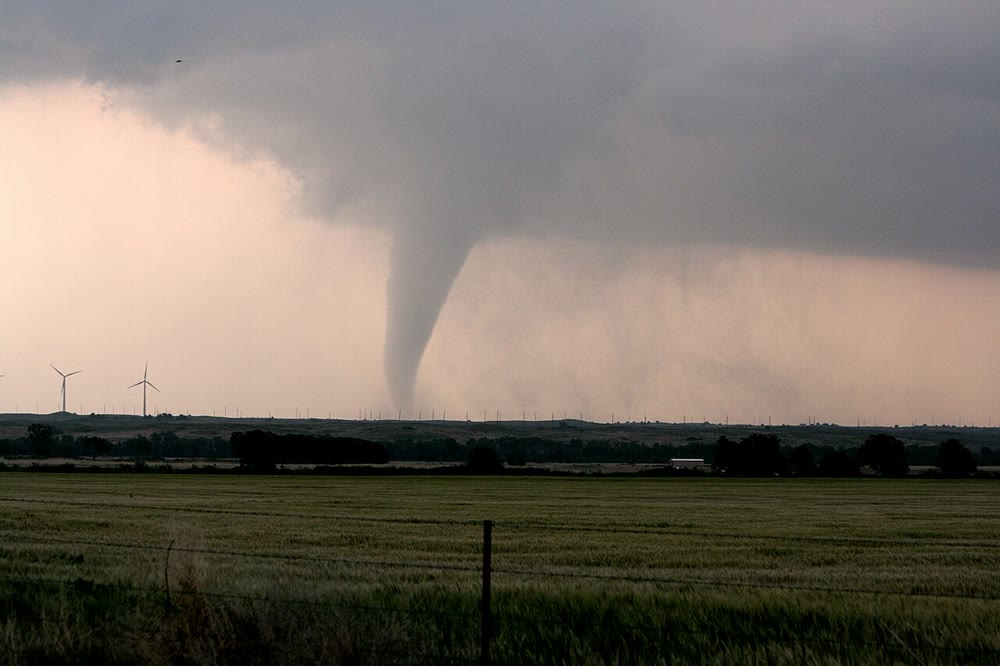
\includegraphics[width=0.62\linewidth]{images/book2/g10-noaa-tornado-kansas.jpg}

{\small Un \omterm{def:g10:storms-and-cyclones:tornado}{tornado} sobre las llanuras de Kansas, en mayo de 2008: el embudo
cuelga de la base de la nube de tormenta. Fotografía: Sean Waugh, NOAA
National Severe Storms Laboratory (dominio público).}
\end{omfigure}

\section{Los ciclones tropicales}

\begin{definition}[Ciclón tropical; ojo; pared del ojo]\label{def:g10:storms-and-cyclones:tropical-cyclone}
Un \emph{ciclón tropical}\index{ciclon tropical@ciclón tropical} es una
tempestad de cientos de kilómetros de diámetro que se forma sobre un mar
tropical cálido alrededor de un centro de bajas presiones, con vientos que
convergen en espiral hacia el centro y bandas de tormentas. Cuando sus
vientos sostenidos alcanzan \num{64}~nudos, unos \qty{119}{km/h}, se le llama
huracán en el Atlántico y en el Pacífico oriental, tifón en el Pacífico
occidental y simplemente ciclón en el océano Índico y en el Pacífico Sur. Su
centro, en calma y casi sin nubes, es el \emph{ojo}\index{ojo}; el anillo de
tormentas altísimas que lo rodea, donde los vientos son más fuertes, es la
\emph{pared del ojo}\index{pared del ojo}.
\end{definition}
% ledger: nhc:sshws

\begin{omfigure}
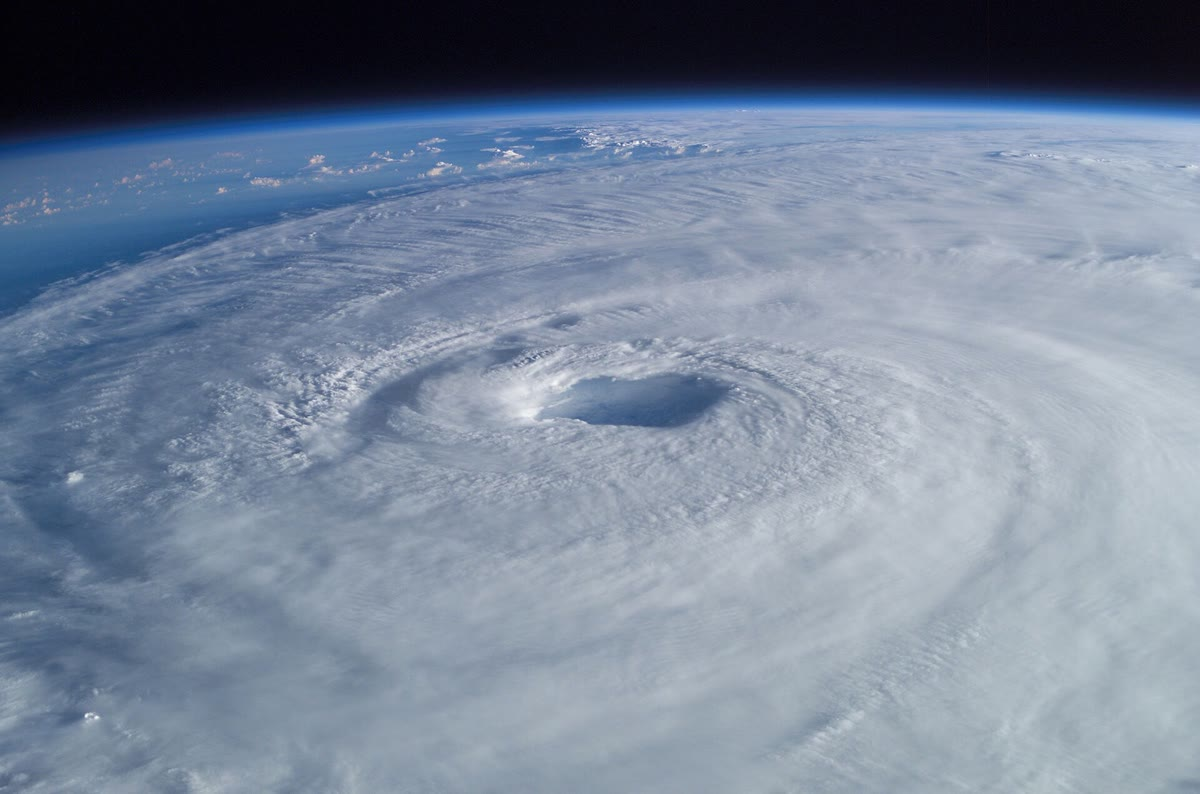
\includegraphics[width=0.78\linewidth]{images/book2/g10-nasa-hurricane-isabel.jpg}

{\small El huracán Isabel, el 15 de septiembre de 2003, fotografiado por un
astronauta desde la Estación Espacial Internacional: el \omterm{def:g10:storms-and-cyclones:tropical-cyclone}{ojo}, la \omterm{def:g10:storms-and-cyclones:tropical-cyclone}{pared del ojo}
y la espiral de nubes que los rodea. Imagen: Mike Trenchard, Earth Sciences
and Image Analysis Laboratory, NASA Johnson Space Center (dominio público).}
\end{omfigure}

Cerca de la superficie del mar, el aire húmedo fluye hacia las bajas
presiones del centro. La rotación de la Tierra desvía el aire en movimiento
hacia la derecha en el hemisferio norte: en lugar de ir directo al centro,
el aire gira a su alrededor, en sentido contrario a las agujas del reloj
visto desde arriba (en el sentido de las agujas del reloj en el hemisferio
sur). Cerca del centro, sube en la \omterm{def:g10:storms-and-cyclones:tropical-cyclone}{pared del ojo}, se condensa y sale por la
parte alta de la tempestad. En el \omterm{def:g10:storms-and-cyclones:tropical-cyclone}{ojo}, un poco de aire desciende, se
calienta y se seca: el cielo se despeja.

\begin{omfigure}
\begin{tikzpicture}[font=\footnotesize, >={Stealth[length=2mm]}]
  \fill[omDef!25] (-6,-0.4) rectangle (6,0);
  \node[anchor=north, omDef!80!black] at (0,-0.05) {mar cálido};
  % rain bands
  \foreach \x/\h in {-5.0/1.6, -3.9/2.2, 3.9/2.2, 5.0/1.6}
    \fill[black!10, draw=black!45] (\x-0.35,0.4) -- (\x-0.3,\h) .. controls (\x-0.15,\h+0.35) and (\x+0.15,\h+0.35) .. (\x+0.3,\h) -- (\x+0.35,0.4) -- cycle;
  % eyewall towers and outflow canopy
  \fill[black!14, draw=black!50] (-2.4,0.4) -- (-2.5,4.0) -- (-5.8,4.3) -- (-5.6,4.7) -- (-1.0,4.9) -- (-0.75,4.0) -- (-0.8,0.4) -- cycle;
  \fill[black!14, draw=black!50] (2.4,0.4) -- (2.5,4.0) -- (5.8,4.3) -- (5.6,4.7) -- (1.0,4.9) -- (0.75,4.0) -- (0.8,0.4) -- cycle;
  % inflow, rise, outflow, eye subsidence
  \draw[->, thick, omThm!80!black] (-5.8,0.2) -- (-1.3,0.2) -- (-1.3,4.3) -- (-4.2,4.45);
  \draw[->, thick, omThm!80!black] (5.8,0.2) -- (1.3,0.2) -- (1.3,4.3) -- (4.2,4.45);
  \draw[->, thick, omDef!80!black] (0,4.3) -- (0,1.0);
  \node[anchor=south, align=center] at (0,5.0) {ojo: aire seco\\que desciende};
  \node[anchor=south east, align=right] at (-2.6,4.95) {pared del ojo};
  \node[anchor=west, align=left] at (-5.95,2.9) {bandas\\de lluvia};
  \node[anchor=north, align=center] at (-3.6,0.15) {entrada de aire húmedo};
  \node[anchor=south east, align=right] at (5.8,4.95) {salida en altura};
  % plan view
  \begin{scope}[shift={(8.4,2.3)}]
    \draw[black!40] (0,0) circle (1.7);
    \foreach \a in {0,90,180,270}
      \draw[->, thick, omThm!80!black, domain=0:200, samples=30, variable=\t]
        plot ({(1.6-0.0045*\t)*cos(\a+\t)}, {(1.6-0.0045*\t)*sin(\a+\t)});
    \fill[white, draw=black!50] (0,0) circle (0.22);
    \node[anchor=north, align=center] at (0,-1.8) {visto desde arriba\\(hemisferio norte)};
  \end{scope}
\end{tikzpicture}

{\small Un \omterm{def:g10:storms-and-cyclones:tropical-cyclone}{ciclón tropical} en corte (esquema, altura muy exagerada): el aire
húmedo entra sobre el mar cálido, sube en la \omterm{def:g10:storms-and-cyclones:tropical-cyclone}{pared del ojo} y en las bandas de
lluvia, y sale por arriba; en el \omterm{def:g10:storms-and-cyclones:tropical-cyclone}{ojo} desciende un poco de aire. Derecha:
visto desde arriba en el hemisferio norte, el aire que entra gira alrededor
del centro en sentido contrario a las agujas del reloj.}
\end{omfigure}

Los ciclones tropicales necesitan un océano cálido: agua de al menos unos
\qty{27}{\degreeCelsius} en superficie, caliente hasta unos \qty{46}{m} de
profundidad. No se forman sobre el propio ecuador, donde la rotación de la
Tierra no imprime ningún giro al aire que entra: una tempestad tiene que
estar al menos a unos \qty{480}{km} del ecuador para que empiece a girar.
% ledger: aoml:formation

\begin{omfigure}
\begin{tikzpicture}
\begin{axis}[ommap, width=\linewidth, xtick={-180,-120,...,180}, ytick={-60,-30,0,30,60},
  ymin=-70, ymax=70, unbounded coords=jump]
\addplot[fill=omLithAlluv, draw=black!45, line width=0.2pt] table {figdata/out/shared-geo-land.dat};
\addplot[omThm!70, line width=0.25pt] table {figdata/out/grade-10-cyclones-tracks.dat};
\addplot[only marks, mark=*, mark size=0.45pt, omDef!90!black] table {figdata/out/grade-10-cyclones-genesis.dat};
\addplot[black!45, dashed, domain=-180:180] {0};
\end{axis}
\end{tikzpicture}

{\small Ciclones tropicales: las trayectorias de todas las tempestades de las
temporadas 2015--2024 (en rojo), y el lugar en el que cada tempestad de las
temporadas 1980--2024 alcanzó por primera vez la intensidad de tormenta
tropical (puntos azules). Datos: IBTrACS v04r01, NOAA National Centers for
Environmental Information.}
\end{omfigure}
% ledger: data:b2-ibtracs (all statistics computed in figdata/grade-10/cyclones.py)

El mapa muestra la regla en acción. De las 3\,888 tempestades de 1980--2024,
solo 24 alcanzaron la intensidad de tormenta tropical a menos de
\qty{5}{\degree} del ecuador. La mayoría se forman entre \qty{10}{\degree} y
\qty{30}{\degree} de latitud, derivan después hacia el oeste con los alisios
y se curvan hacia los polos, donde el mar frío las debilita. El Atlántico
Sur, más frío y menos favorable, solo tuvo tres en 45 años. En un año medio
se forman unos 87 ciclones tropicales, siete de cada diez en el hemisferio
norte, y algo más de la mitad alcanzan la intensidad de huracán.

\begin{proposition}[La fuente de energía de un ciclón tropical]\label{prop:g10:storms-and-cyclones:energy}
Un \omterm{def:g10:storms-and-cyclones:tropical-cyclone}{ciclón tropical} saca su energía del mar cálido: el \omterm{def:g10:earth-energy-budget:latent-heat}{calor latente} que
absorbe la evaporación en la superficie del mar se libera en la \omterm{def:g10:storms-and-cyclones:tropical-cyclone}{pared del
ojo} y en las bandas de lluvia cuando el vapor se condensa. Un huracán medio
libera así unos \qty{6e14}{W}; solo una pequeña parte, unos
\qty{1.5e12}{W}, se convierte en energía cinética de sus vientos.
\end{proposition}
% ledger: aoml:energy

\begin{proof}[Justificación]
Un huracán medio deja caer \qty{1.5}{cm} de lluvia al día sobre un círculo
de radio \qty{665}{km}, de área $\pi \times (665\,000)^2 \approx
\qty{1.39e12}{m^2}$: \qty{2.1e10}{m^3}, es decir, \qty{2.1e13}{kg}, de agua
al día. Cada kilogramo que se condensa libera unos \qty{2.5}{MJ}:
$2.1\times10^{13}
\times 2.5\times10^6 \approx \qty{5.2e19}{J}$ al día, es
decir, $5.2\times10^{19}/86\,400 \approx \qty{6.0e14}{W}$. La potencia de los
vientos es una estimación a partir de campos de viento medidos, tomada de la
misma fuente.
\end{proof}

La tempestad funciona como un motor: toma calor en la superficie cálida del
mar, lo cede en lo alto, en el aire frío de las capas superiores, y una
parte de la diferencia se convierte en movimiento del viento. Por eso un
\omterm{def:g10:storms-and-cyclones:tropical-cyclone}{ciclón tropical} se debilita deprisa cuando pasa sobre tierra firme o sobre
agua fría: pierde su aporte de agua que se evapora.

\section{Intensidad, vientos y mareas de tempestad}

\begin{definition}[Escala de Saffir--Simpson]\label{def:g10:storms-and-cyclones:scale}
La \emph{escala de Saffir--Simpson}\index{escala de Saffir--Simpson}
clasifica los huracanes en cinco categorías según su viento sostenido
máximo; las categorías 3 a 5 son huracanes \emph{mayores}.
\end{definition}

\begin{center}
\small
\begin{tabular}{cccc}
\hline
categoría & nudos & \unit{m/s} & \unit{km/h} \\
\hline
1 & 64--82 & 33--42 & 119--153 \\
2 & 83--95 & 43--49 & 154--177 \\
3 & 96--112 & 49--58 & 178--208 \\
4 & 113--136 & 58--70 & 209--251 \\
5 & 137 o más & 70 o más & 252 o más \\
\hline
\end{tabular}
\end{center}
% ledger: nhc:sshws (m/s converted with 1 knot = 1852/3600 m/s)

Cuanto más profundas son las bajas presiones del centro, más fuertes son los
vientos que soplan a su alrededor: la diferencia de presión entre el centro
y los alrededores es lo que empuja el aire hacia dentro.

\begin{omfigure}
\begin{tikzpicture}
\begin{axis}[omrecord, width=0.86\linewidth, height=6.2cm, xmin=15, xmax=100,
  ymin=860, ymax=1015, xlabel={viento sostenido máximo (\unit{m/s})},
  ylabel={presión central mínima (\unit{hPa})},
  tick label style={font=\small}, label style={font=\small}]
\foreach \w in {32.92, 42.70, 49.39, 58.13, 70.48}
  \edef\temp{\noexpand\draw[black!55, densely dashed] (axis cs:\w,860) -- (axis cs:\w,1015);}\temp
\addplot[only marks, mark=*, mark size=0.6pt, omDef!80!black, opacity=0.6] table[x=wind_ms, y=pmin_hpa] {figdata/out/grade-10-cyclones-scatter.dat};
\addplot[omThm!85!black, thick] table[x=wind_ms, y=pmin_hpa] {figdata/out/grade-10-cyclones-fit.dat};
\node[font=\scriptsize, black!60] at (axis cs:37.8,1008) {1};
\node[font=\scriptsize, black!60] at (axis cs:46.0,1008) {2};
\node[font=\scriptsize, black!60] at (axis cs:53.8,1008) {3};
\node[font=\scriptsize, black!60] at (axis cs:64.3,1008) {4};
\node[font=\scriptsize, black!60] at (axis cs:76,1008) {5};
\end{axis}
\end{tikzpicture}

{\small Cada punto es un \omterm{def:g10:storms-and-cyclones:tropical-cyclone}{ciclón tropical} de las temporadas 2000--2024: su
viento sostenido más fuerte y su presión central más baja. La recta es el
mejor ajuste lineal: unos \qty{1.6}{hPa} menos por cada metro por segundo de
más. Líneas grises discontinuas: los límites de las categorías de
Saffir--Simpson (numeradas arriba). Datos: IBTrACS v04r01, NOAA NCEI.}
\end{omfigure}
% ledger: data:b2-ibtracs, nhc:sshws (fit computed in figdata/grade-10/cyclones.py)

El récord de las tempestades de 1980--2024 del archivo pertenece al huracán
Patricia, frente a la costa pacífica de México en octubre de 2015: vientos
sostenidos de 185 nudos, unos \qty{95}{m/s}, y una presión central de
\qty{872}{hPa}.
% ledger: data:b2-ibtracs

\begin{definition}[Marea de tempestad]\label{def:g10:storms-and-cyclones:storm-surge}
Una \emph{marea de tempestad}\index{marea de tempestad} es la subida del mar
por encima de su nivel normal, sin contar la marea, causada por una
tempestad: el viento amontona el agua contra la costa, y las bajas presiones
dejan que el mar se abombe bajo la tempestad.
\end{definition}

\begin{proposition}[El abombamiento por la presión]\label{prop:g10:storms-and-cyclones:bulge}
Bajo una tempestad cuya presión central está $\Delta p$ hectopascales por
debajo de la de sus alrededores, el mar sube unos $\Delta p$ centímetros.
\end{proposition}

\begin{proof}
Muy por debajo de la superficie, la presión tiene que ser la misma bajo la
tempestad y fuera de ella; si no, el agua fluiría. El aire que hay sobre la
tempestad pesa $\Delta p$ menos; una columna de agua de mar de altura $h$ lo
compensa si $\rho g h = \Delta p$. Para $\Delta p = \qty{1}{hPa} = \qty{100}{Pa}$, con $\rho = \qty{1025}{kg/m^3}$ y $g = \qty{9.81}{m/s^2}$:
$h = 100/(1025
\times 9.81) \approx \qty{0.0099}{m}$, alrededor de \qty{1}{cm}.
\end{proof}
% ledger: noaa:seawater-1025, nasa:aquarius-density, const:gn

El abombamiento es la parte menor de la mayoría de las \omterm{def:g10:storms-and-cyclones:storm-surge}{mareas de tempestad}:
bajo una presión central de \qty{920}{hPa}, \qty{90}{hPa} por debajo de sus
alrededores, es de unos \qty{0.9}{m}. El viento hace el resto, empujando el
agua hacia la orilla, sobre todo sobre un fondo marino ancho y poco
profundo. Si llega con la marea alta, una \omterm{def:g10:storms-and-cyclones:storm-surge}{marea de tempestad} de varios metros
puede inundar costas bajas hasta muy tierra adentro.

\begin{omfigure}
\begin{tikzpicture}[font=\footnotesize, >={Stealth[length=2mm]}]
  \def\surf{(0,0) .. controls (1.5,0) and (2.2,0.5) .. (3.0,0.5) .. controls (3.8,0.5) and (4.6,0.4) .. (5.6,0.5) .. controls (7.2,0.65) and (8.8,1.0) .. (10.25,1.3)}
  \fill[omDef!20] (0,-1.6) -- \surf -- (8.8,-1.6) -- cycle;
  \draw[thick, omDef!80!black] \surf;
  \draw[black!50, dashed] (0,0) -- (9.6,0);
  \node[anchor=north west, black!60] at (0.1,-0.05) {nivel normal del mar};
  \fill[omExo!30, draw=black!60] (8.8,-1.6) -- (10.4,1.6) -- (12.4,1.7) -- (12.4,-1.6) -- cycle;
  \foreach \x in {10.9,11.7} \draw[fill=white, draw=black!60] (\x,1.63) rectangle (\x+0.45,2.03) (\x-0.05,2.03) -- (\x+0.225,2.28) -- (\x+0.5,2.03);
  \draw[<->, omThm!80!black] (3.0,0) -- (3.0,0.5);
  \node[anchor=south east, omThm!80!black, align=right] at (2.8,0.6) {abombamiento bajo\\las bajas presiones};
  \draw[<->, omThm!80!black] (9.4,0) -- (9.4,1.12);
  \node[anchor=south, omThm!80!black, align=center] at (8.9,1.75) {sobreelevación por el\\viento contra la costa};
  \foreach \y in {2.9,3.4} \draw[->, thick, black!60] (4.0,\y) -- (6.4,\y);
  \node[anchor=south] at (5.2,3.45) {viento hacia tierra};
  \node[anchor=south, align=center] at (3.0,1.9) {centro de\\la tempestad};
  \draw[black!40] (3.0,1.9) -- (3.0,0.65);
\end{tikzpicture}

{\small Una \omterm{def:g10:storms-and-cyclones:storm-surge}{marea de tempestad} (esquema, alturas muy exageradas): el mar sube
alrededor de \qty{1}{cm} por cada hectopascal de bajas presiones bajo la
tempestad, y el viento que sopla hacia tierra amontona el agua contra la
costa.}
\end{omfigure}

\begin{omfigure}
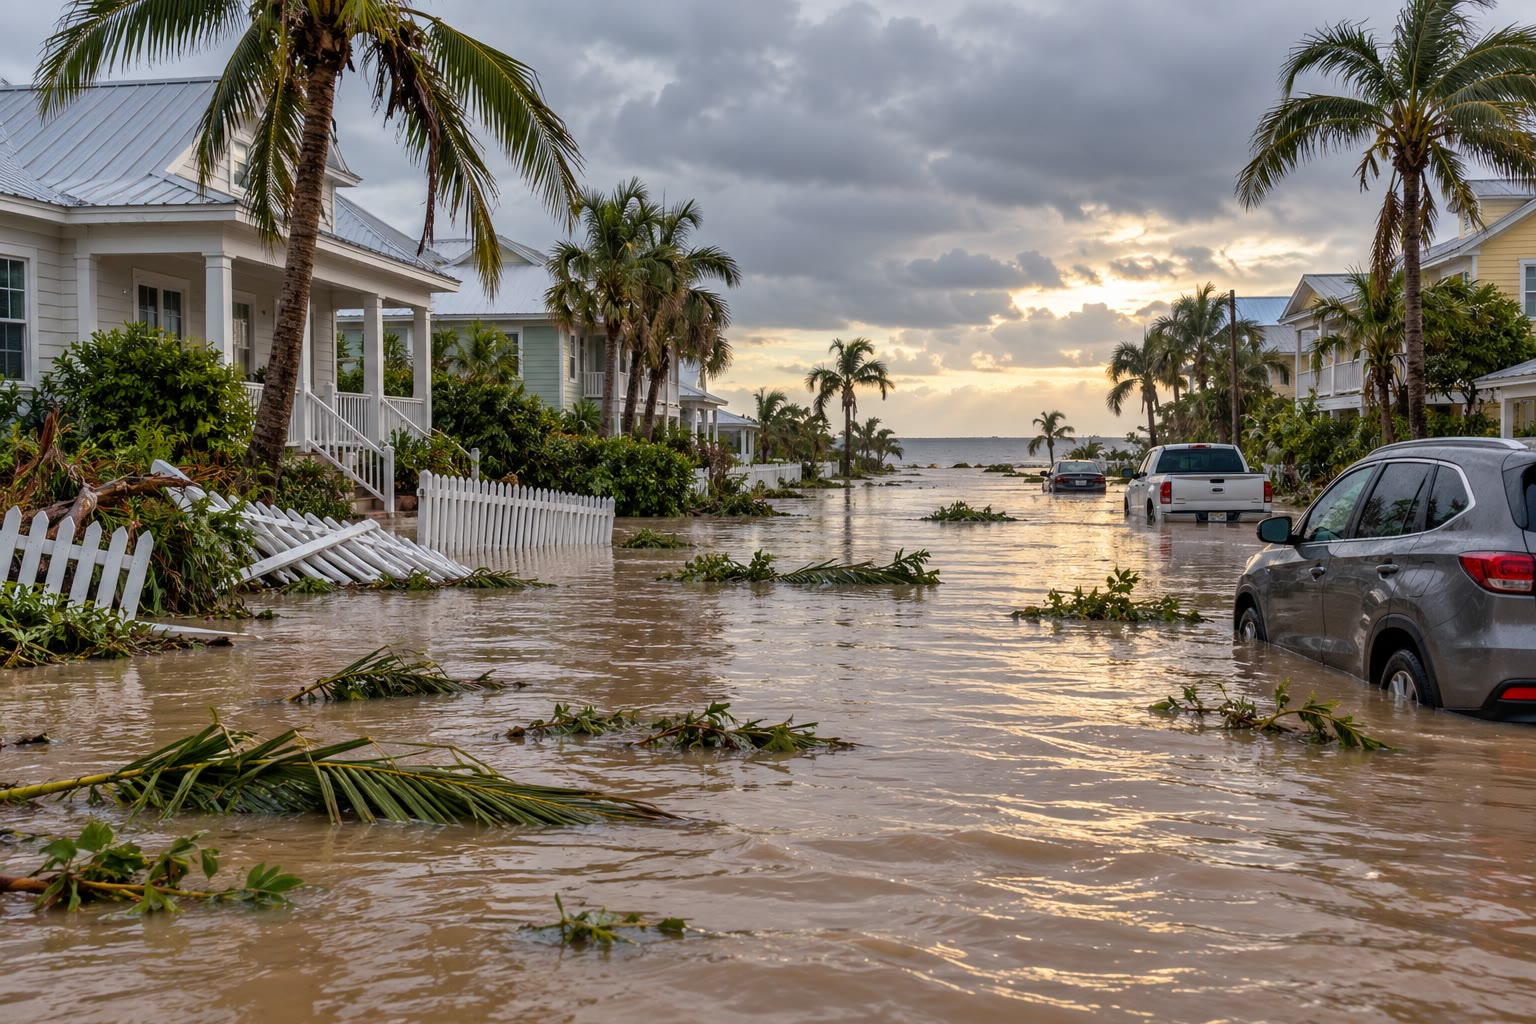
\includegraphics[width=0.7\linewidth]{images/book2/ai/g10-flooded-street.jpg}

{\small Una calle costera la mañana después de una \omterm{def:g10:storms-and-cyclones:storm-surge}{marea de tempestad}: agua de
mar, palmeras rotas y vallas arrancadas.}
\end{omfigure}

\section{Ejercicios}

\begin{exercise}[$\star$]\label{exo:g10:storms-and-cyclones:1}
Define una \omterm{def:g10:storms-and-cyclones:thunderstorm}{tormenta eléctrica} y un \omterm{def:g10:storms-and-cyclones:lightning}{rayo}. ¿Qué produce el sonido del trueno?
\end{exercise}

\begin{exercise}[$\star$]\label{exo:g10:storms-and-cyclones:2}
Define un \omterm{def:g10:storms-and-cyclones:tropical-cyclone}{ciclón tropical}, su \omterm{def:g10:storms-and-cyclones:tropical-cyclone}{ojo} y la \omterm{def:g10:storms-and-cyclones:tropical-cyclone}{pared del ojo}. ¿Dónde son más fuertes
sus vientos?
\end{exercise}

\begin{exercise}[$\star$]\label{exo:g10:storms-and-cyclones:3}
¿En qué categoría de Saffir--Simpson está un huracán con vientos sostenidos
de \num{70}~nudos? ¿Y de \num{120}~nudos? ¿Y de \num{140}~nudos? ¿Cuáles de
ellos son huracanes mayores?
\end{exercise}

\begin{exercise}[$\star$]\label{exo:g10:storms-and-cyclones:4}
Cuentas \num{9} segundos entre un relámpago y su trueno, y después \num{15}
segundos para el relámpago siguiente. ¿A qué distancia estaba cada uno? ¿Se
está acercando la tormenta?
\end{exercise}

\begin{exercise}[$\star$]\label{exo:g10:storms-and-cyclones:5}
Explica por qué un árbol aislado en medio de un campo es un refugio peligroso
durante una tormenta, y adónde deberías ir en su lugar.
\end{exercise}

\begin{exercise}[$\star\star$]\label{exo:g10:storms-and-cyclones:6}
Un nudo son \qty{1852}{m} por hora. Convierte \num{64}~nudos y
\num{137}~nudos a \unit{m/s} y a \unit{km/h}.
\end{exercise}

\begin{exercise}[$\star\star$]\label{exo:g10:storms-and-cyclones:7}
En la Tierra se producen 44 \omterm{def:g10:storms-and-cyclones:lightning}{rayos} por segundo. ¿Cuántos son en un día, y en
un año?
\end{exercise}

\begin{exercise}[$\star\star$]\label{exo:g10:storms-and-cyclones:8}
Un huracán tiene una presión central de \qty{935}{hPa} en unos alrededores a
\qty{1010}{hPa}. ¿Qué altura tiene el abombamiento del mar por la presión
bajo él?
\end{exercise}

\begin{exercise}[$\star\star$]\label{exo:g10:storms-and-cyclones:9}
Con el mapa de trayectorias, describe dónde se forman los ciclones tropicales
y adónde van después de formarse. ¿Por qué no aparecen sobre el propio
ecuador?
\end{exercise}

\begin{exercise}[$\star\star$]\label{exo:g10:storms-and-cyclones:10}
La recta del gráfico presión--viento es $p \approx 1031 - 1.56\,v$ ($p$ en
\unit{hPa}, $v$ en \unit{m/s}). ¿Qué presión central da para el límite
inferior de la categoría 5, \qty{70}{m/s}? ¿Y para una tempestad de
\qty{40}{m/s}?
\end{exercise}

\begin{exercise}[$\star\star$]\label{exo:g10:storms-and-cyclones:11}
Explica por qué un \omterm{def:g10:storms-and-cyclones:tropical-cyclone}{ciclón tropical} se debilita deprisa cuando pasa sobre
tierra firme, y por qué se debilita sobre agua fría.
\end{exercise}

\begin{exercise}[$\star\star\star$]\label{exo:g10:storms-and-cyclones:12}
La velocidad del sonido en el aire es $\sqrt{1.4\,R\,T/M}$, con $R =
\qty{8.314}{J.mol^{-1}.K^{-1}}$, $T$ en kelvin y $M =
\qty{0.02897}{kg/mol}$. Calcúlala a \qty{0}{\degreeCelsius} y a
\qty{30}{\degreeCelsius}. Para un retraso de \qty{9}{s}, ¿cuánto difieren las
dos distancias? ¿Es suficiente la regla de los ``\qty{3}{s} por kilómetro''?
\end{exercise}

\begin{exercise}[$\star\star\star$]\label{exo:g10:storms-and-cyclones:13}
En una costa se mide una \omterm{def:g10:storms-and-cyclones:storm-surge}{marea de tempestad} de \qty{4.0}{m} cuando llega a
tierra un huracán con una presión central de \qty{940}{hPa} (alrededores a
\qty{1010}{hPa}). ¿Qué parte de la subida se debe al abombamiento por la
presión, y qué parte al viento? Si llega con la marea alta, \qty{1.5}{m} por
encima del nivel medio del mar, ¿hasta qué altura sobre el nivel medio del
mar llega el agua?
\end{exercise}

\begin{exercise}[$\star\star\star$]\label{exo:g10:storms-and-cyclones:14}
Un \omterm{def:g10:storms-and-cyclones:tornado}{tornado} gira con vientos de \qty{90}{m/s} a \qty{100}{m} de su eje, y un
huracán, con vientos de \qty{60}{m/s} en una \omterm{def:g10:storms-and-cyclones:tropical-cyclone}{pared del ojo} situada a
\qty{30}{km} del centro. ¿Cuánto tarda el aire en dar una vuelta en cada
caso? Compáralos.
\end{exercise}

\begin{exercise}[$\star\star\star$]\label{exo:g10:storms-and-cyclones:15}
De los 3\,888 ciclones tropicales de 1980--2024, 24 alcanzaron la intensidad
de tormenta tropical a menos de \qty{5}{\degree} del ecuador, 414 a menos de
\qty{10}{\degree} y 121 más allá de \qty{30}{\degree}. Calcula los tres
porcentajes. La franja situada a menos de \qty{5}{\degree} del ecuador ocupa
alrededor del \qty{9}{\percent} de la superficie terrestre: ¿qué cabría
esperar si la latitud no importara, y qué concluyes?
\end{exercise}

\section{Problema: el motor térmico de un huracán}

\begin{problem}[{Problema de fin de semana --- de la lluvia de un día a la
potencia del viento}]
\label{pb:g10:storms-and-cyclones:1}
% ledger: aoml:energy, nist:water-latent, earth:Rmean, ipcc:budget-toa (all results computed in figdata/grade-10/cyclones.py or from the rounded data below)
Un huracán medio deja caer \qty{1.5}{cm} de lluvia al día sobre un círculo
de radio \qty{665}{km}. Usa un \omterm{def:g10:earth-energy-budget:latent-heat}{calor latente} de \qty{2.5}{MJ/kg}, una
densidad del agua de \qty{1000}{kg/m^3}, \qty{86400}{s} en un día, y la
potencia de los vientos de un huracán medio, \qty{1.5e12}{W}.

\medskip
\noindent\textbf{Parte I --- La lluvia de un día.}
\begin{enumerate}
  \item Calcula el área del círculo.
  \item Calcula el volumen de lluvia que cae sobre él en un día.
  \item Exprésalo en kilómetros cúbicos.
  \item Calcula su masa.
\end{enumerate}

\medskip
\noindent\textbf{Parte II --- El calor liberado.}
\begin{enumerate}[resume]
  \item Calcula el \omterm{def:g10:earth-energy-budget:latent-heat}{calor latente} que libera en un día la condensación de
        esta agua.
  \item Conviértelo en una potencia.
  \item La Tierra entera absorbe unos \qty{1.22e17}{W} de luz solar
        (\cref{ch:g10:earth-energy-budget}). ¿Qué fracción de esa cantidad
        libera un solo huracán?
  \item La luz solar absorbida media es de \qty{240}{W/m^2}. Calcula la luz
        solar que absorbe la superficie de la tempestad y compárala con el
        \omterm{def:g10:earth-energy-budget:latent-heat}{calor latente} de la tempestad.
  \item ¿Qué muestra esta comparación sobre dónde se reunió la energía de
        la tempestad?
\end{enumerate}

\medskip
\noindent\textbf{Parte III --- De dónde viene el agua.}
\begin{enumerate}[resume]
  \item ¿Qué masa de agua tiene que evaporarse cada día para alimentar esta
        lluvia?
  \item La evaporación media de la superficie terrestre transporta
        \qty{82}{W/m^2}. ¿Sobre qué superficie aportaría la evaporación media
        el \omterm{def:g10:earth-energy-budget:latent-heat}{calor latente} de la tempestad? Compárala con la superficie de la
        tempestad.
  \item Con la tabla de contenidos de saturación del
        \cref{ch:g10:why-clouds-form}, compara el agua que contiene el aire
        saturado a \qty{28}{\degreeCelsius} y a \qty{20}{\degreeCelsius}.
  \item Explica por qué los ciclones tropicales solo se forman sobre mares
        cálidos.
  \item Explica por qué se debilitan sobre tierra firme.
\end{enumerate}

\medskip
\noindent\textbf{Parte IV --- El viento.}
\begin{enumerate}[resume]
  \item Calcula la energía cinética que reciben los vientos en un día.
  \item Convierte el límite inferior de la categoría 3, \num{96}~nudos, a
        \unit{m/s} (\num{1}~nudo = \qty{1852}{m/h}).
  \item El aire cercano a la superficie del mar tiene una densidad de unos
        \qty{1.16}{kg/m^3}. Calcula la energía cinética de un metro cúbico de
        ese aire que se mueve a esa velocidad.
  \item Compara el \omterm{def:g10:earth-energy-budget:latent-heat}{calor latente} liberado en un día con la energía de los
        vientos en un día.
  \item ¿En qué se convierte el resto del calor liberado?
  \item ¿Qué fracción del calor liberado por la condensación se convierte en
        viento?
\end{enumerate}
\end{problem}
